%include part: see main.beamer.tex and main.article.tex
%include common packages and settings
\usepackage{etex} %эта магическая херь избавляет от переполнения регистров TeX а!!!

\mode<article>{\usepackage{fullpage}}
\mode<presentation>{
    \usetheme{Madrid} %%Boadilla,Madrid,AnnArbor,CambridgeUS,Malmoe,Singapore,Berlin
    \useoutertheme{shadow}
} 

\usepackage[utf8]{inputenc}
\usepackage[russian]{babel}
\usepackage{indentfirst}
\usepackage{graphicx}

\usepackage{amsmath}
\usepackage{amsfonts}
\usepackage{amsthm}
\usepackage{algorithm}
\usepackage{algorithmic}

\usepackage[all]{xy}

\date{Лекция по дисциплине <<дискретная математика>>\\(\today)}
\author[М.~М.~Шихов]{Михаил Шихов \\ \texttt{\underline{m.m.shihov@gmail.com}}}

%для рисования графов пакетом xy-pic
\entrymodifiers={++[o][F-]}

%для псевдокода алгоритмов (algorithm,algorithmic)
\renewcommand{\algorithmicrequire}{\textbf{Вход:}}
\renewcommand{\algorithmicensure}{\textbf{Выход:}}
\renewcommand{\algorithmiccomment}[1]{// #1}
\floatname{algorithm}{Псевдокод}



\title[Отношения и функции]{Отношения и функции}


\begin{document}

%титул и содержание статьи
\mode<article>{\maketitle\tableofcontents}

%титул и содержание презентации
\frame<presentation>{\titlepage}
\begin{frame}<presentation>
    \frametitle{Содержание}
    \tableofcontents
\end{frame}


\section{Отношения}


\subsection{Определения}

\begin{frame}
    \frametitle{Отношения}
    
    \begin{definition}
        $n$-местным \alert{отношением} или $n$-местным \alert{предикатом} $P$ на множествах $A_1, A_2, \ldots, A_n$ называется любое подмножество прямого произведения $A_1\times A_2\times \cdots\times A_n$.
        \[
            P\subseteq A_1\times A_2\times \cdots\times A_n.
        \]
    \end{definition}
    
    \begin{definition}
        Элементы $x_1,x_2,\ldots,x_n$ (где $x_1\in A_1,x_2\in A_2,\ldots,x_n\in A_n$) связаны соотношением $P$:
        \[
            P(x_1,x_2,\ldots,x_n)
        \] 
        тогда и только тогда, когда $(x_1,x_2,\ldots,x_n)\in P$.
    \end{definition}
\end{frame}

\begin{frame}
    \frametitle{$P\subseteq A_1\times A_2\times \cdots\times A_n$}
    \framesubtitle{Частные виды отношений}
    
    \begin{itemize}
        \item $n=1$. $P$ --- \alert{унарное} отношение или \alert{свойство}. 
        
        \item $n=2$. $P$ --- \alert{бинарное} отношение. Если $P\subseteq A\times B$ и $(x,y)\in P$, вместо $P(x,y)$ также пишут $x\,P\,y$.
        \begin{example}[Бинарное отношение нестрогого включения $\subseteq$]
            Вместо <<$\subseteq(x, y)$>> пишут $x \subseteq y$
        \end{example}
        
        \item $P\subseteq A^n$ --- $n$-местный предикат (отношение) \alert{на множестве} $A$. 
        \begin{example}[Бинарное отношение \alert{на} $\mathbb{R}$. Здесь $x,y\in\mathbb{R}$]
            \[x \leq y\]
        \end{example}
    \end{itemize}
\end{frame}

\subsection{Бинарные отношения}

\begin{frame}
    \frametitle{Способы задать бинарное $P\subseteq A\times B$}
    
    \begin{itemize}
        \item множеством упорядоченных пар: $\{(a,b)|P(a,b)\}$;
        \item точками в декартовой системе координат;
        \item ориентированным графом;
        \item матрицей смежности;
        \item списком смежности. 
    \end{itemize}
\end{frame}

\begin{frame}
    \frametitle{Способ задать бинарное $P\subseteq A\times B$}
    \framesubtitle{Множество точек в декартовой системе координат}
    
    \begin{example}
        Дано: $A=B=\{w,x,y,z\}$. $P\subseteq \{w,x,y,z\}^2$.
        
        Пусть: $P=\{(w,x),(x,y),(y,z),(z,w),(w,y),(y,w),(w,w),(y,y)\}$.
    \end{example}
    
    \begin{center}
        \only<1>{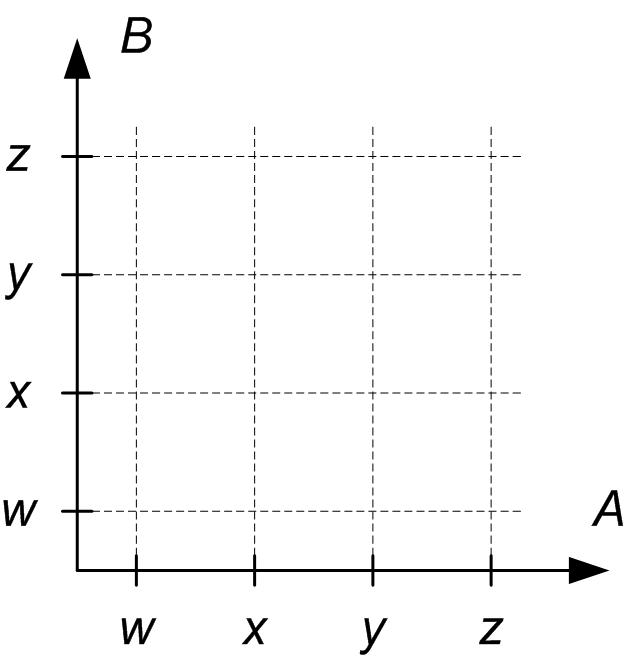
\includegraphics[width=.35\textwidth]{fig/p2decartE}}
        \only<2>{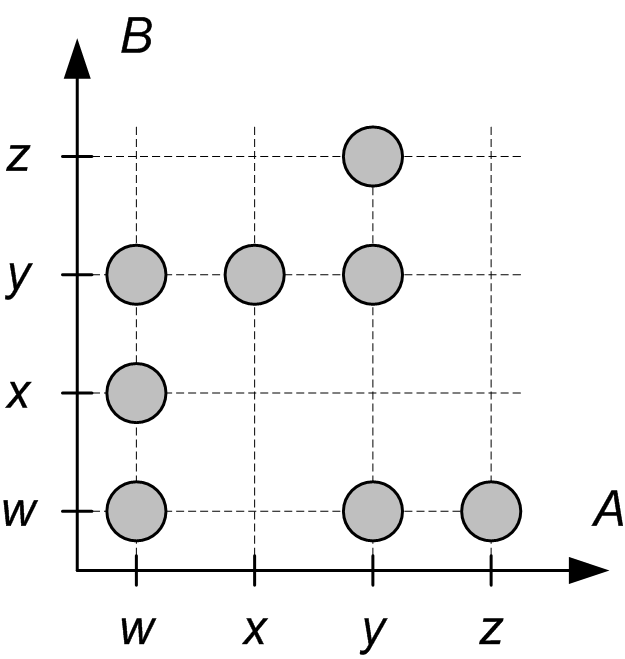
\includegraphics[width=.35\textwidth]{fig/p2decartA}}
    \end{center}
\end{frame}

\begin{frame}
    \frametitle{Способ задать бинарное $P\subseteq A\times B$}
    \framesubtitle{Ориентированный граф}
    
    Вершинам соответствуют элементы $A\cup B$, а дугам $(a,b)\in P$.
    
    \begin{example}
        Дано: $A=B=\{w,x,y,z\}$. $P\subseteq \{w,x,y,z\}^2$.
        
        Пусть: $P=\{(w,x),(x,y),(y,z),(z,w),(w,y),(y,w),(w,w),(y,y)\}$.
    \end{example}
    
    \[
        {\xymatrix{
            x \only<2>{ \ar@{->}[r] }
                &y \only<2>{ \ar@{->}@(u,r)[] \ar@{->}[d] \ar@{->}@/^/[dl] }
                    \\
            w \only<2>{ \ar@{->}@(d,l)[] \ar@{->}[u] \ar@{->}@/^/[ur] }
                &z \only<2>{ \ar@{->}[l] }
        }}
    \]
\end{frame}

\begin{frame}
    \frametitle{Способ задать бинарное $P\subseteq A\times B$}
    \framesubtitle{Матрица смежности $[P]$}
    
    Пусть $A=\{a_1,\ldots,a_m\}$, $B=\{b_1,\ldots,b_n\}$. Элементы $[P]_{m\times n}$:
    \[
        [P]_{i,j}=
        \begin{cases}
            1,  &\text{если $(a_i,b_j)\in P$},\\
            0,  &\text{если $(a_i,b_j)\not\in P$}.
        \end{cases}
    \]
    
    \begin{example}
        Дано: $A=B=\{w,x,y,z\}$. $P\subseteq \{w,x,y,z\}^2$.
        
        Пусть: $P=\{(w,x),(x,y),(y,z),(z,w),(w,y),(y,w),(w,w),(y,y)\}$.
    \end{example}
    
    \[
        [P]=
        \begin{array}{c|cccc}
             &            w &            x &            y &            z \\ \hline
            w&\uncover<2>{1}&\uncover<2>{1}&\uncover<2>{1}&\uncover<2>{0}\\
            x&\uncover<2>{0}&\uncover<2>{0}&\uncover<2>{1}&\uncover<2>{0}\\
            y&\uncover<2>{1}&\uncover<2>{0}&\uncover<2>{1}&\uncover<2>{1}\\
            z&\uncover<2>{1}&\uncover<2>{0}&\uncover<2>{0}&\uncover<2>{0}
        \end{array}
        \uncover<2>{=
            \begin{pmatrix}
                1&1&1&0 \\
                0&0&1&0 \\
                1&0&1&1 \\
                1&0&0&0
            \end{pmatrix}
        }.
    \]
\end{frame}
    
\begin{frame}
    \frametitle{Способ задать бинарное $P\subseteq A\times B$}
    \framesubtitle{Список смежности}
    
    Если $a\in A$, то множество смежных с $a$ элементов: $\{b|b\in B, P(a,b)\}$.
    
    \begin{example}
        Дано: $A=B=\{w,x,y,z\}$. $P\subseteq \{w,x,y,z\}^2$.
        
        Пусть: $P=\{(w,x),(x,y),(y,z),(z,w),(w,y),(y,w),(w,w),(y,y)\}$.
    \end{example}
    
    \[
        \begin{array}{c|l}
            \hline\hline
            a\in A&\{b|b\in B, P(a,b)\} \\ 
            \hline\hline
            w   &\uncover<2>{\{w,y,x\}}  \\
            x   &\uncover<2>{\{y\}}      \\
            y   &\uncover<2>{\{z,w,y\}}  \\
            z   &\uncover<2>{\{w\}}
        \end{array}
    \]
\end{frame}

\begin{frame}
    \frametitle{Частные случаи бинарных отношений на множестве $A$}
    \framesubtitle{$P\subseteq A^2$}
    
    \begin{itemize}
        \item \alert{тождественное} отношение (или \alert{диагональ}): $I_A=\{(x,x)|x\in A\}$;
        \item \alert{универсальное} (или \alert{полное}) отношение: $U_A=A^2$.
    \end{itemize}
\end{frame}

\begin{frame}
    \frametitle{Область определения и область значений}
    
    Для бинарного отношения $P\subseteq A\times B$.
    \begin{itemize}
        \item \alert{Областью определения} называется множество $\delta_P=\{a|(a,b)\in P\}$.
        \item \alert{Областью значений} называется множество $\rho_P=\{b|(a,b)\in P\}$.
    \end{itemize}
\end{frame}

\begin{frame}
    \frametitle{Дополнение и обратное отношение}
    
    \alert{Дополнением} отношения $P\subseteq A\times B$ называется отношение
    \[\overline{P}=\{(a,b)|(a,b)\in A\times B\land (a,b)\not\in P\}.\]

    \alert{Обратным} к $P$ отношением называется отношение
    \[P^{-1}=\{(b,a)|(a,b)\in P\}.\]
\end{frame}

\begin{frame}
    \frametitle{Композиция отношений}
    \framesubtitle{$P_1\subseteq A\times B, P_2\subseteq B\times C, P_1\cdot P_2\subseteq A\times C$}
    
    \alert{Композиции} (\emph{произведение}) отношений $P_1\subseteq A\times B$ и $P_2\subseteq B\times C$:
    \[
        \begin{split}
            P_1\cdot P_2 = P_1P_2 = \\
            = \{(a,c)|a\in A\land c\in C\land (\exists b\in B \left((a,b)\in P_1\land (b,c)\in P_2\right))\}
        \end{split}
    \]
\end{frame}

\begin{frame}
    \frametitle{Пример композиции}
    
    \begin{example}[$A=\{1,2\}$, $B=\{x,y\}$, $C=\{3,4,5\}$]
        $P\subseteq A\times B$, $Q=B\times C$: 
        \[P=\{(1,x),(1,y),(2,y)\}, Q=\{(x,3),(x,4),(y,4),(y,5)\}.\]
    \end{example}
    
    \uncover<2>{
        \[
            \raisebox{3\height}{
                {\xymatrix@=.7pc{
                    1 \ar@{->}[r] \ar@{->}[dr]
                        &x  \ar@{->}[r] \ar@{->}[dr] 
                            &3 
                                \\
                    2 \ar@{->}[r]
                        &y \ar@{->}[r] \ar@{->}[dr]
                            &4 
                                \\
                    *{}
                        &*{}
                            &5 
                }}
            }
            \begin{array}{l}
                1\,P\,x\land x\,Q\,3\Rightarrow (1,3)\in PQ\\
                1\,P\,x\land x\,Q\,4\Rightarrow (1,4)\in PQ\\
                1\,P\,y\land y\,Q\,4\Rightarrow (1,4)\in PQ\\
                1\,P\,y\land y\,Q\,5\Rightarrow (1,5)\in PQ\\
                2\,P\,y\land y\,Q\,4\Rightarrow (2,4)\in PQ\\
                2\,P\,y\land y\,Q\,5\Rightarrow (2,5)\in PQ\\
                \\
                PQ=\{(1,3),(1,4),(1,5), \\
                (2,4),(2,5)\}
            \end{array}        
            \raisebox{3\height}{
                {\xymatrix@=.7pc{
                    1 \ar@{->}[r] \ar@{->}[dr] \ar@{->}[ddr]
                        &3 
                            \\
                    2 \ar@{->}[r] \ar@{->}[dr]
                        &4 
                            \\
                    *{}
                        &5 
                }}
            }
        \]
    }
\end{frame}
	
\begin{frame}
    \frametitle{Степень бинарного отношения на множестве $A$}
    \framesubtitle{$P\subseteq A^2$}
    
    \[
        P^n=
        \begin{cases}
            P^{0}=I_A,              &n=0;\\
            P^{n}=P^{n-1}\cdot P,   &n>0.
        \end{cases}
    \]
    т.е.
    \[
        P^n=\underbrace{P\cdot P\cdot\ldots\cdot P}_n.
    \]
\end{frame}

\begin{frame}
    \frametitle{Операции на матрицах смежности}
    \framesubtitle{Композиция}
    
    Пусть $A=\{a_1,\ldots,a_m\}$, $B=\{b_1,\ldots,b_n\}$, $C=\{c_1,\ldots,c_k\}$.
    
    $P\subseteq A\times B$, $Q=B\times C$ заданы матрицами $[P]_{m\times n}$, $[Q]_{n\times k}$.

    Тогда $[PQ]_{m\times k} = [P]_{m\times n}\cdot [Q]_{n\times k}$. Здесь $[P]_{m\times n}\cdot [Q]_{n\times k}$ --- \alert{логическое} или \alert{булево} произведение матриц.

    Каждый элемент матрицы композиции получается по формуле
    \[
        [PQ]_{i,j}=\bigvee_{l=1}^{n} \big([P]_{i,l}\land [Q]_{l,j}\big),
    \]
    где $1\leq i\leq m$, $1\leq j\leq k$.
\end{frame}

\begin{frame}
    \frametitle{Пример композиции}
    \framesubtitle{Булево произведение матриц смежности}
    
	\[
		[P]_{2\times 2}=
		\begin{array}{c|cc}
			  & x & y \\ \hline
			1 & 1 & 1 \\
			2 & 0 & 1
		\end{array}=
		\begin{pmatrix}
			1&1\\
			0&1
		\end{pmatrix},\,
		[Q]_{2\times 3}=
		\begin{array}{c|ccc}
			  & 3 & 4 & 5 \\ \hline
			x & 1 & 1 & 0 \\
			y & 0 & 1 & 1 
		\end{array}=
		\begin{pmatrix}
			1&1&0 \\
			0&1&1 
		\end{pmatrix}.
	\]

	И матрица композиции:
	\[
		[PQ]_{2\times 3}=
		[P]_{2\times 2}\cdot [Q]_{2\times 3}=
		\begin{pmatrix}
			1&1\\
			0&1
		\end{pmatrix}\cdot
		\begin{pmatrix}
			1&1&0 \\
			0&1&1 
		\end{pmatrix}=
		\begin{array}{c|ccc}
			  &             3            & 4            & 5  \\ \hline
			1 & \uncover<2>{1}&\uncover<2>{1}&\uncover<2>{1} \\
			2 & \uncover<2>{0}&\uncover<2>{1}&\uncover<2>{1}
		\end{array}.
	\]
    \uncover<2>{
        Например, элемент $[PQ]_{2,1}$ получается так:
        \[
            [PQ]_{2,1}=\begin{pmatrix}0&1\end{pmatrix}\cdot\begin{pmatrix}1\\0\end{pmatrix}=
            (0\land 1)\lor(1\land0) = 0.
        \]
    }
\end{frame}

\begin{frame}
    \frametitle{Операции на матрицах смежности}
    \framesubtitle{Объединение и пересечение отношений}
    
    Пусть $A=\{a_1,\ldots,a_m\}$, $B=\{b_1,\ldots,b_n\}$.
    
    $P,Q\subseteq A\times B$, $[P]_{m\times n}$, $[Q]_{m\times n}$.
    
    Тогда матрицы:
    \begin{itemize}
        \item объединения отношений
        \[
            [P\cup Q]_{i,j}=\uncover<2>{ [P]_{i,j}\lor [Q]_{i,j} };
        \]
        
        \item пересечение отношений
        \[
            [P\cap Q]_{i,j}=\uncover<2>{ [P]_{i,j}\land [Q]_{i,j} }.
        \]
    \end{itemize}
\end{frame}

\begin{frame}
    \frametitle{Операции на матрицах смежности}
    \framesubtitle{Дополнение и обратное отношение}
    
    $P$ задано матрицей $[P]_{m\times n}$.
    
    Тогда:
    \begin{itemize}
        \item дополнение $P$
        \[
            [\overline{P}]_{i,j}=\overline{ [P]_{i,j} };
        \]
        
        \item обратное к $P$ отношение
        \[
            [P^{-1}]_{n\times m}=([P]_{m\times n}])^{T}, 
        \]
        где каждый элемент $[P^{-1}]_{j,i}=[P]_{i,j}$.
    \end{itemize}
\end{frame}


\section{Функции}

\subsection{Определения}

\begin{frame}
    \frametitle{Функция}
    
    \begin{definition}
        Отношение $f\subseteq A\times B$ называется \alert{функцией} или \alert{отображением} из множества $A$ в множество $B$, если область определения $\delta_f=A$, область значений $\rho_f\subseteq B$ и из $(x,y_1)\in f$, $(x,y_2)\in f$ следует $y_1=y_2$. 
        \begin{itemize}
            \item Если вместо $\delta_f=A$ выполняется $\delta_f\subset A$, то $f$ называется \alert{частичной} функцией.
        \end{itemize}
    \end{definition}

    \[
        \begin{array}{c|c}
            \begin{array}{c}
                {
                    \xymatrix@=.7pc{
                        x_1  \ar@{->}[r] \ar@{->}[dr]
                            &y_1
                                \\
                        x_2 \ar@{->}[r]
                            &y_2 
                                \\
                        x_3 \ar@{->}[r]
                            &y_3
                    }
                }\\
                \uncover<2>{ \text{Отношение, но не функция!} }
            \end{array}
            &
            \begin{array}{c}
                {
                    \xymatrix@=.7pc{
                        x_1  \ar@{->}[r]
                            &y_1
                                \\
                        x_2 \ar@{->}[dr]
                            &y_2 
                                \\
                        x_3 
                            &y_3
                    }    
                }\\
                \uncover<2>{ \text{Частичная функция} }
            \end{array}
        \end{array}
    \]
\end{frame}

\begin{frame}
    \frametitle{Обозначения}
    
    Функция из $A$ в $B$ обозначается так:
    \[f:A\to B.\]

    Если $(x,y)\in f$, то пишется $y=f(x)$ или $f:x\mapsto y$ (понимается как <<функция $f$ ставит в соответствие элементу $x$ элемент $y$>>).
    
    Понятие функции легко обобщается до случая $n$-аргументов:
    \[
        \begin{matrix}
        f:X_1\times \ldots \times X_n \to Y; &y = f(x_1,\ldots,x_n); &f:(x_1,\ldots,x_n)\mapsto y.
        \end{matrix}
    \]
    
    Функцию, как частный случай отношения, можно задать явным перечислением элементов:
    \[\uncover<2>{\oplus} = \{(0,0)\mapsto 0, (0,1)\mapsto 1, (1,0)\mapsto 1, (1,1)\mapsto 0\}\]
\end{frame}


\subsection{Типы функций}

\begin{frame}
    \frametitle{Типы функций}
    \framesubtitle{Инъекция и сюръекция}
    
    \begin{definition}
        Функция $f:A\to B$ называется \alert{разнозначной}, функцией $A$ в $B$ или \alert{инъекцией}, если $f^{-1}$ --- \alert{частичная} функция. То есть справедливо, что для любых двух элементов из области определения $x_1,x_2\in\delta_f$ из $x_1\neq x_2$ следует $f(x_1)\neq f(x_2)$. Обозначают инъекцию $f:A\xrightarrow{\text{в}} B$.
    \end{definition}

    \begin{definition}
        Функция $f:A\to B$ называется функцией $A$ на $B$ или \alert{сюръекцией} если область значений $\rho_f=B$. Обозначают сюръекцию $f:A\xrightarrow{\text{на}} B$.
    \end{definition}
\end{frame}

\begin{frame}
    \frametitle{Инъекция и сюръекция}
    \framesubtitle{Пример}
    
    \[
        \begin{array}{c|c|c}
            \begin{array}{c}
                {
                    \xymatrix@=.7pc{
                        x_1  \ar@{->}[r]
                            &y_1
                                \\
                        x_2 \ar@{->}[dr]
                            &y_2 
                                \\
                        *{}
                            &y_3
                    }
                }\\
                \uncover<2> {
                    \text{Инъекция}\\
                    f:X\xrightarrow{\text{в}} Y\\
                    \text{Не сюръекция!}
                }
            \end{array}
            &
            \begin{array}{c}
                {
                    \xymatrix@=.7pc{
                        x_1  \ar@{->}[r]
                            &y_1
                                \\
                        x_2 \ar@{->}[r]
                            &y_2 
                                \\
                        x_3 \ar@{->}[ur]
                            &*{}
                    }    
                }\\
                \uncover<2> {
                    \text{Сюръекция}\\
                    f:X\xrightarrow{\text{на}} Y\\
                    \text{Не инъекция!}
                }
            \end{array}
            &
            \begin{array}{c}
                {
                    \xymatrix@=.7pc{
                        x_1 \ar@{->}[r]
                            &y_1
                                \\
                        x_2 \ar@{->}[ur]
                            &y_2 
                                \\
                        x_3 \ar@{->}[ur]
                            &y_3
                    }    
                }\\
                \uncover<2> {
                    f:X\to Y\\
                    \text{Не сюръекция!}\\
                    \text{Не инъекция!}
                }
            \end{array}        
        \end{array}
    \]
\end{frame}

\begin{frame}
    \frametitle{Биекция}
    
    \begin{definition}
        Функция $f$ называется \alert{взаимно однозначным соответствием} между множествами $A$ и $B$ или \alert{биекцией}, если она является одновременно и инъекцией и сюръекцией. Обозначают биекцию так: $f:A\leftrightarrow B$.
    \end{definition}

    \[
        \begin{array}{c}
            {
                \xymatrix@=.7pc{
                    x_1  \ar@{->}[r]
                        &y_1
                            \\
                    x_2 \ar@{->}[dr]
                        &y_2 
                            \\
                    x_3 \ar@{->}[ur]
                        &y_3
                }
            }\\
            \text{Биекция $f:X\leftrightarrow Y$}\\
            \text{Cюръекция и инъекция одновременно!}
        \end{array}
    \]
    
    Биекцию $f:A\leftrightarrow A$ называют \emph{подстановкой} множества $A$.
\end{frame}

\begin{frame}
    \frametitle{Задача}
    \framesubtitle{Определить типы функций}
    
    \only<1>{
        \begin{center}
            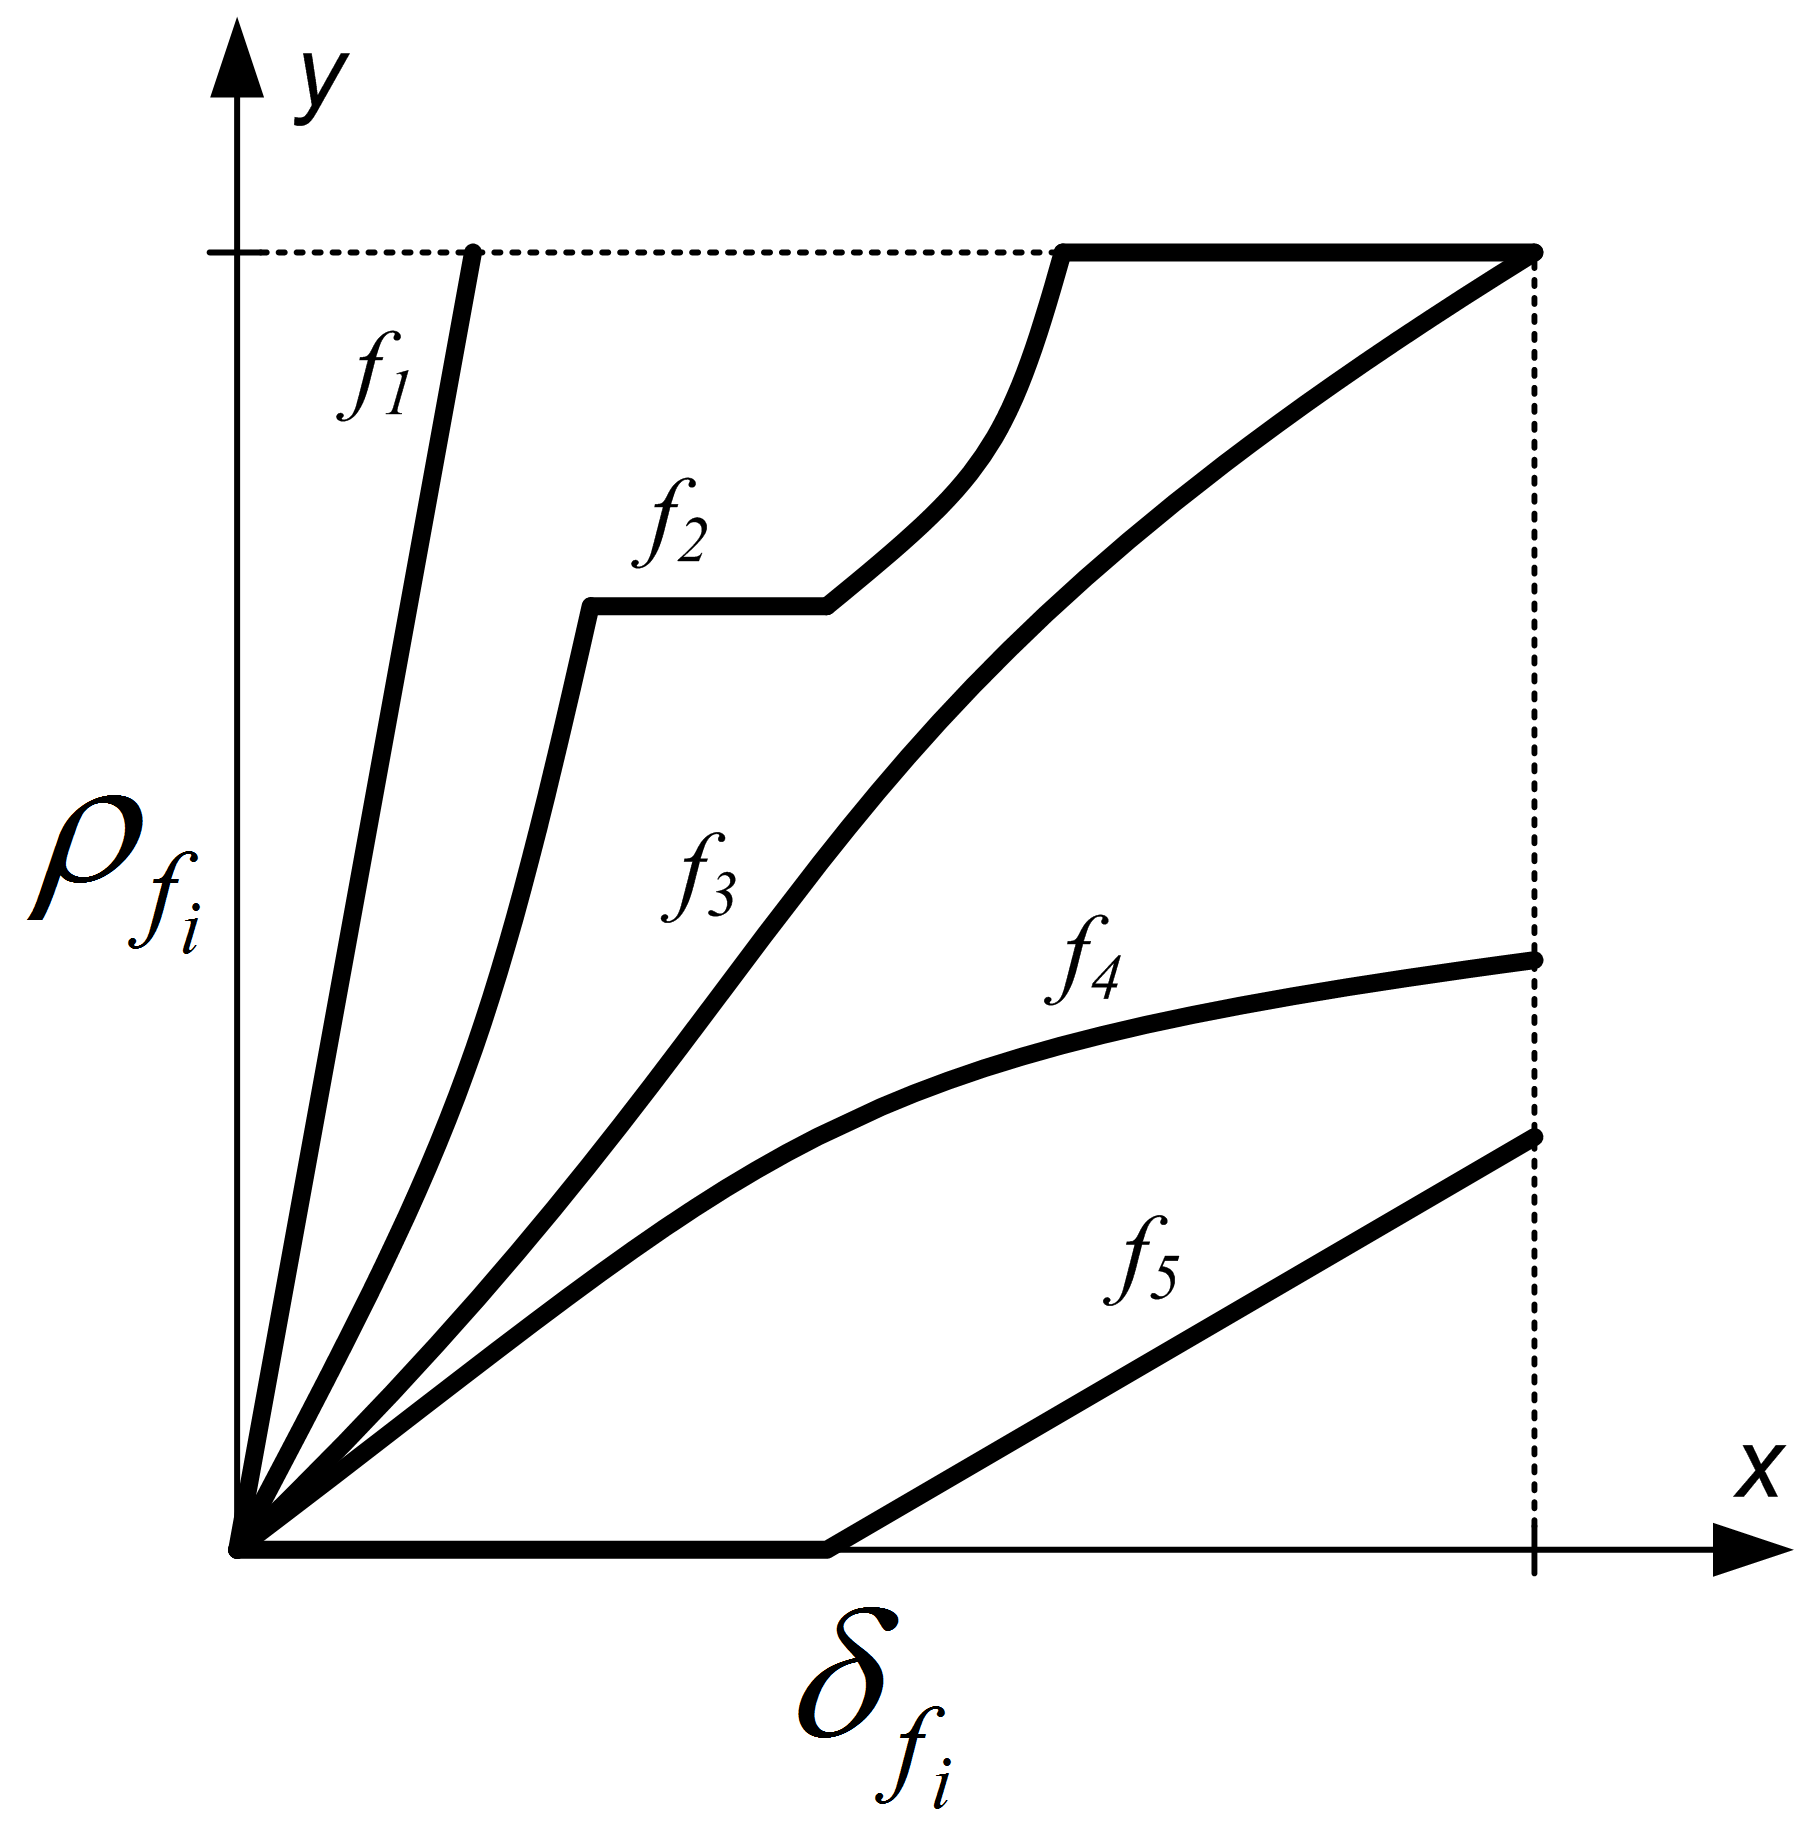
\includegraphics[width=.55\textwidth]{fig/functionProps}
        \end{center} 
    }
    \only<2>{
        \begin{itemize}
            \item $f_1$ на данной области определения не является функцией! Это \alert{частичная} функция.
            \item $f_2$ \alert{сюръективна}, но \alert{не инъективна}.
            \item $f_3$ \alert{биективна} (стало быть и \alert{инъективна} и \alert{сюръективна}).
            \item $f_4$ \alert{инъективна}, но \alert{не сюръективна}.
            \item $f_5$ \alert{не инъективна} и \alert{не сюръективна}.
        \end{itemize}
    }
\end{frame}


\begin{frame}
    \frametitle{Частные случаи функций}
    
    \begin{itemize}
        \item Функция $f:\mathbb{N}\to B$ называется \alert{последовательностью}.

        \item Функция $f:A^n\to B$ называется \alert{$n$-местной функцией} из $A$ в $B$. 

        \item Функция $f:A^n\to A$ называется \alert{$n$-местной алгебраической операцией} на множестве $A$. При:
        \begin{itemize}
            \item $n=1$ операция называется \alert{унарной}; 
            \item $n=2$ --- \alert{бинарной};
            \item $n>2$ --- $n$-арной. 
            \item $n=0$ операция $f:A^0\to A$ есть множество $\{(\emptyset,a)\}$ для некоторого $a\in A$. В этом случае операцию обычно называют \alert{константой} и отождествляют с $a$.
        \end{itemize}
    \end{itemize}
\end{frame}



\appendix


\begin{frame}
    \frametitle{В заключение}
    
    Отношения и функции являются важнейшими понятиями математики и активно используются для решения практических задач. Для углубленного изучения материала рекомендуются \cite{bib:sudoplatov:discrmath, bib:haggard:discrmathprogrammer}.
\end{frame}


\begin{frame}[allowframebreaks]{Библиография}
    \bibliographystyle{gost780u}
    \bibliography{./../../bibliobase}
\end{frame}

\end{document}